\documentclass[a4,12pt]{scrartcl}

\usepackage[a4paper,top=0.5in,bottom=0.5in]{geometry}
\usepackage{graphicx}
\usepackage{caption}
\usepackage{relsize}
\usepackage{fancyhdr}

\usepackage[pdftex,pdfpagemode=UseNone]{hyperref}



%% set pdf properties
\hypersetup{%
    pdftitle={Supplemental Material: Hybrid Data Visualization Based On Depth Complexity Histogram Analysis},
    pdfauthor={Paper ID},
%    pdfauthor={Stefan Lindholm, Martin Falk, Erik Sund\'en, Alexander Bock, Anders Ynnerman, and Timo Ropinski},
    pdfsubject={Supplemental Material}
}

\newcommand{\ab}{\mbox{A-buffer}}

\newcommand{\stencil}{ppAO}
\newcommand{\dloop}{ppDP}


\begin{document}
\thispagestyle{empty}

\section*{{\smaller Supplemental Material}\\ Hybrid Data Visualization Based On Depth Complexity Histogram Analysis}
\label{sec:suppl}

\begin{figure}[h!]
  \centering
  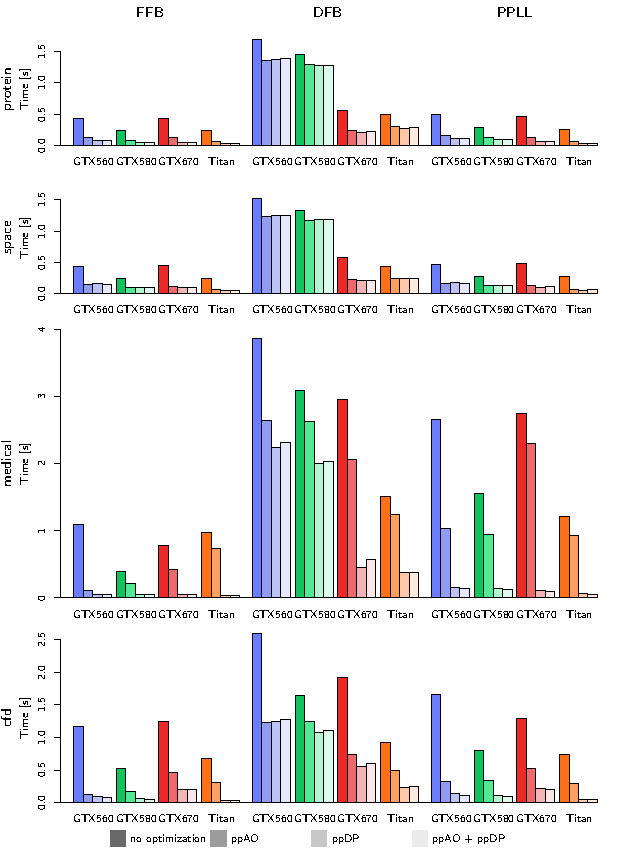
\includegraphics[scale=1.5]{suppl-plot-performance}
  \caption{\label{fig:perfsuppl}%
    Performance comparison with our proposed \stencil{} and \dloop{} components.
    Columns represent the different \ab{} implementations in combination with our components (none, \stencil{}, \dloop{}, \stencil{} and \dloop{} combined).
  }
\end{figure}

\end{document}

%%% Local Variables: 
%%% mode: latex
%%% TeX-master: t
%%% End: 
